% Author: Izaak Neutelings (January 2021)
\documentclass[border=3pt,tikz]{standalone}
\usepackage{amsmath}
\usepackage{etoolbox} % ifthen
\usepackage{tikz}
\usepackage{ifthen}
\usetikzlibrary{arrows.meta} % for arrow size
\tikzset{>=latex} % for LaTeX arrow head

\colorlet{xcol}{blue!70!black}
\colorlet{vcol}{green!60!black}
\colorlet{myred}{red!80!black}
\colorlet{myblue}{blue!80!black}
\colorlet{mypurple}{blue!50!red!80}
\colorlet{metalcol}{blue!25!black!30!white}
\tikzstyle{metal}=[draw=metalcol!10!black,rounded corners=0.1,
  top color=metalcol,bottom color=metalcol!80!black,shading angle=10]
\tikzstyle{ring}=[metalcol!20!black,double=metalcol!70!black,double distance=1.2,line width=0.3]
\tikzstyle{rope}=[brown!20!black,double=brown!70!black,
  double distance=0.8,line width=0.1] %very thick,line cap=round
\tikzstyle{wood}=[draw=brown!80!black,rounded corners=0.1,
  top color=brown!80,bottom color=brown!80!black!80,shading angle=10]
%\tikzstyle{myarr}=[-{Latex[length=3,width=2]},vcol!40]
%\tikzstyle{mydoublearr}=[{Latex[length=3,width=2]}-{Latex[length=3,width=2]},vcol!40]

\def\L{6.0}
\def\t{0.12}
\def\H{0.22}   % mount height
\def\h{0.12}   % fret height
\def\r{0.05}   % fret radius
\def\w{0.18}   % fret width
\def\A{0.5*\h} % amplitude
\def\mount#1{
  \draw[metal] ({(1-#1)*\L},0)++(160:\r) arc(160:20:\r)
    -- ({(1-#1)*\L+\w/2},-\H) --++ (-\w,0) -- cycle;
}
\def\fret#1{
  \def\x{(1-#1)*\L}
  \def\xf{\L-#1*\L-0.57*\w}
  %\draw[fill=pink!60!white,line width=0.1,rounded corners=1]
  %  ({\L-#1*\L-1.5*\w},0.033) rectangle++ (0.7*\w,-1.8*\h)
  %  ({\L-#1*\L-2.2*\w},0.033) rectangle++ (0.7*\w,-1.8*\h);
  \draw[fill=pink!60!white,line width=0.1]
    ({\xf},0.035) circle({0.5*\w} and {0.4*\w});
  \draw[pink!80!black!30,fill=pink!90!black!11,line width=0.1]
    ({\xf},0.035)++(170:{0.47*\w} and {0.4*\w})
      to[out=10,in=170]++ ({2*cos(10)*0.47*\w},0) to[out=125,in=55] cycle;
  \draw[metal] ({(1-#1)*\L},\h-\H)++(160:\r) arc(160:20:\r)
    -- ({\x+\w/2},-\H) --++ (-\w,0) -- cycle;
}
\def\guitar{
  \clip (-2.3*\w,2.35*\A) rectangle (1.28*\L,-3.3*\H); % ensure same canvas height
  \draw[wood] (-2*\w,-\H) rectangle (\L+2*\w,-1.6*\H);
  \mount{0}
  \mount{1}
}
\def\wave#1{
  \def\lam{2*#1*\L} % wavelength
  \def\om{360/(\lam)} % omega (degrees)
  \def\a{(1-#1)*\L}
  \ifthenelse{\lengthtest{#1 pt > 0.9 pt}}{
    \draw[dashed,samples=100,smooth,variable=\x,domain=\a:\L]
      plot(\x,{-\A*sin(\om*(\x-\a))-0.03});
    \draw[rope,samples=100,smooth,variable=\x,domain=0:\L]
      plot(\x,{\A*sin(\om*(\x-\a))});
  }{
    \draw[dashed,samples=100,smooth,variable=\x,domain=\a:\L]
      plot(\x,{-\A*sin(\om*(\x-\a))-0.025+0.026/(#1*\L)*(\x-\L)});
    \draw[rope,samples=100,smooth,variable=\x,domain=\a:\L]
      (0,0) -- (\L-#1*\L-0.46*\w,-0.054) to[out=-2,in=187]
      (\L-#1*\L-0.0145,-0.0275) -- plot(\x,{\A*sin(\om*(\x-\a))+0.0265/(#1*\L)*(\x-\L)});
  }
}

\begin{document}

% STANDING WAVE ON STRING
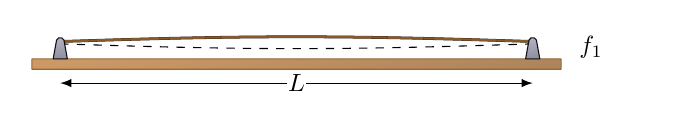
\begin{tikzpicture}
  \draw[<->] (\L,-2.4*\H) --++ (-\L,0)
    node[midway,fill=white,inner sep=0.5,scale=0.9] {$L$};
  \node[below=2,right,scale=0.9] at (1.08*\L,0) {$f_1$};
  \wave{1}
  \guitar
\end{tikzpicture}

% 4/5 - major third
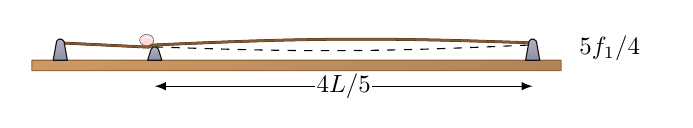
\begin{tikzpicture}
  \draw[<->] (\L,-2.5*\H) --++ (-4*\L/5,0)
    node[midway,fill=white,inner sep=0.5,scale=0.9] {$4L/5$};
  \node[below=2,right,scale=0.9] at (1.08*\L,0) {$5f_1/4$};
  \wave{0.8}
  \guitar
  \fret{0.8}
\end{tikzpicture}

% 3/4 - perfect fourth
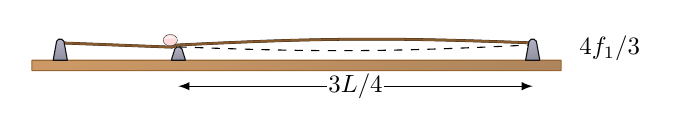
\begin{tikzpicture}
  \draw[<->] (\L,-2.5*\H) --++ (-3*\L/4,0)
    node[midway,fill=white,inner sep=0.5,scale=0.9] {$3L/4$};
  \node[below=2,right,scale=0.9] at (1.08*\L,0) {$4f_1/3$};
  \wave{0.75}
  \guitar
  \fret{0.75}
\end{tikzpicture}

% OCTAVE UP
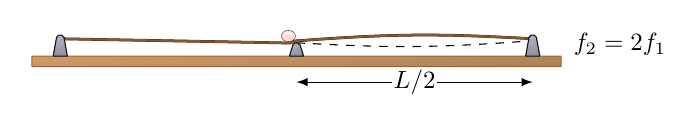
\begin{tikzpicture}
  \draw[<->] (\L,-2.5*\H) --++ (-\L/2,0)
    node[midway,fill=white,inner sep=0.5,scale=0.9] {$L/2$};
  \wave{0.5}
  \guitar
  \node[below=2,right=-2,scale=0.9] at (1.08*\L,0) {$f_2=2f_1$};
  \fret{0.5}
\end{tikzpicture}


\end{document}